% ═════════════════════════════════════════════════════════════════════════════
\section{Results and Discussion}
\label{sec:results}

\subsection{Exploratory Data Analysis}

Table~\ref{tab:desc_stats} reports descriptive statistics for all four return
series over the aligned sample of 2,448 observations. CS2 is the most volatile
asset at 114.56\% annualised, exceeding Bitcoin (69.87\%), consistent with the
first part of H3. The correlation matrix (Table~\ref{tab:correlation}) shows
near-zero contemporaneous correlations between CS2 and all three benchmarks
($r_{\text{CS2,BTC}} = {-}0.016$, $r_{\text{CS2,SP500}} = 0.000$,
$r_{\text{CS2,Gold}} = 0.011$), constituting direct evidence against H1. ADF
tests reject the unit root null at the 1\% level for all series, confirming
that log returns are stationary and no further differencing is required.

\begin{table}[H]
\centering
\caption{Descriptive Statistics --- Daily Log Returns}
\label{tab:desc_stats}
\begin{tabular}{lrrrrr}
\hline
Asset    & Mean (\%) & Std Dev (\%) & Skewness & Ex.\ Kurtosis & Ann.\ Vol.\ (\%) \\
\hline
CS2      & 0.009 & 7.217 & $-$0.37 &  3.82 & 114.56 \\
S\&P 500 & 0.041 & 1.133 & $-$0.80 & 15.74 &  17.98 \\
Bitcoin  & 0.203 & 4.401 & $-$0.63 &  9.07 &  69.87 \\
Gold     & 0.026 & 0.927 & $-$0.06 &  3.77 &  14.71 \\
\hline
\end{tabular}
\end{table}

\begin{table}[H]
\centering
\caption{Correlation Matrix --- Daily Log Returns}
\label{tab:correlation}
\begin{tabular}{lrrrr}
\hline
         & CS2      & S\&P 500 & Bitcoin  & Gold  \\
\hline
CS2      &  1.000   &  0.000   & $-$0.016 & 0.011 \\
S\&P 500 &  0.000   &  1.000   &  0.213   & 0.020 \\
Bitcoin  & $-$0.016 &  0.213   &  1.000   & 0.084 \\
Gold     &  0.011   &  0.020   &  0.084   & 1.000 \\
\hline
\end{tabular}
\end{table}

\begin{figure}[H]
  \centering
  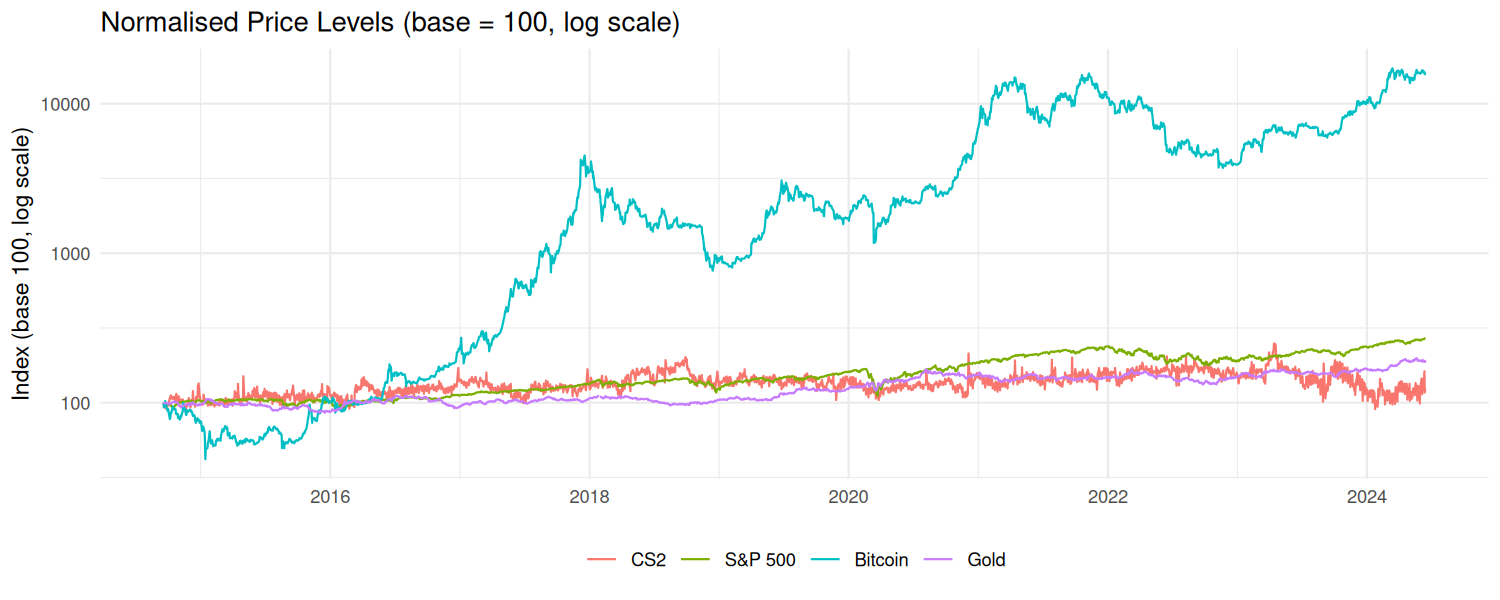
\includegraphics[width=\linewidth]{../images/eda/levels.png}
  \caption{Normalised price levels --- CS2 index, S\&P~500, Bitcoin, and Gold
    (2013--2024, rebased to 100 at start of common sample; log scale).}
  \label{fig:levels}
\end{figure}

\begin{figure}[H]
  \centering
  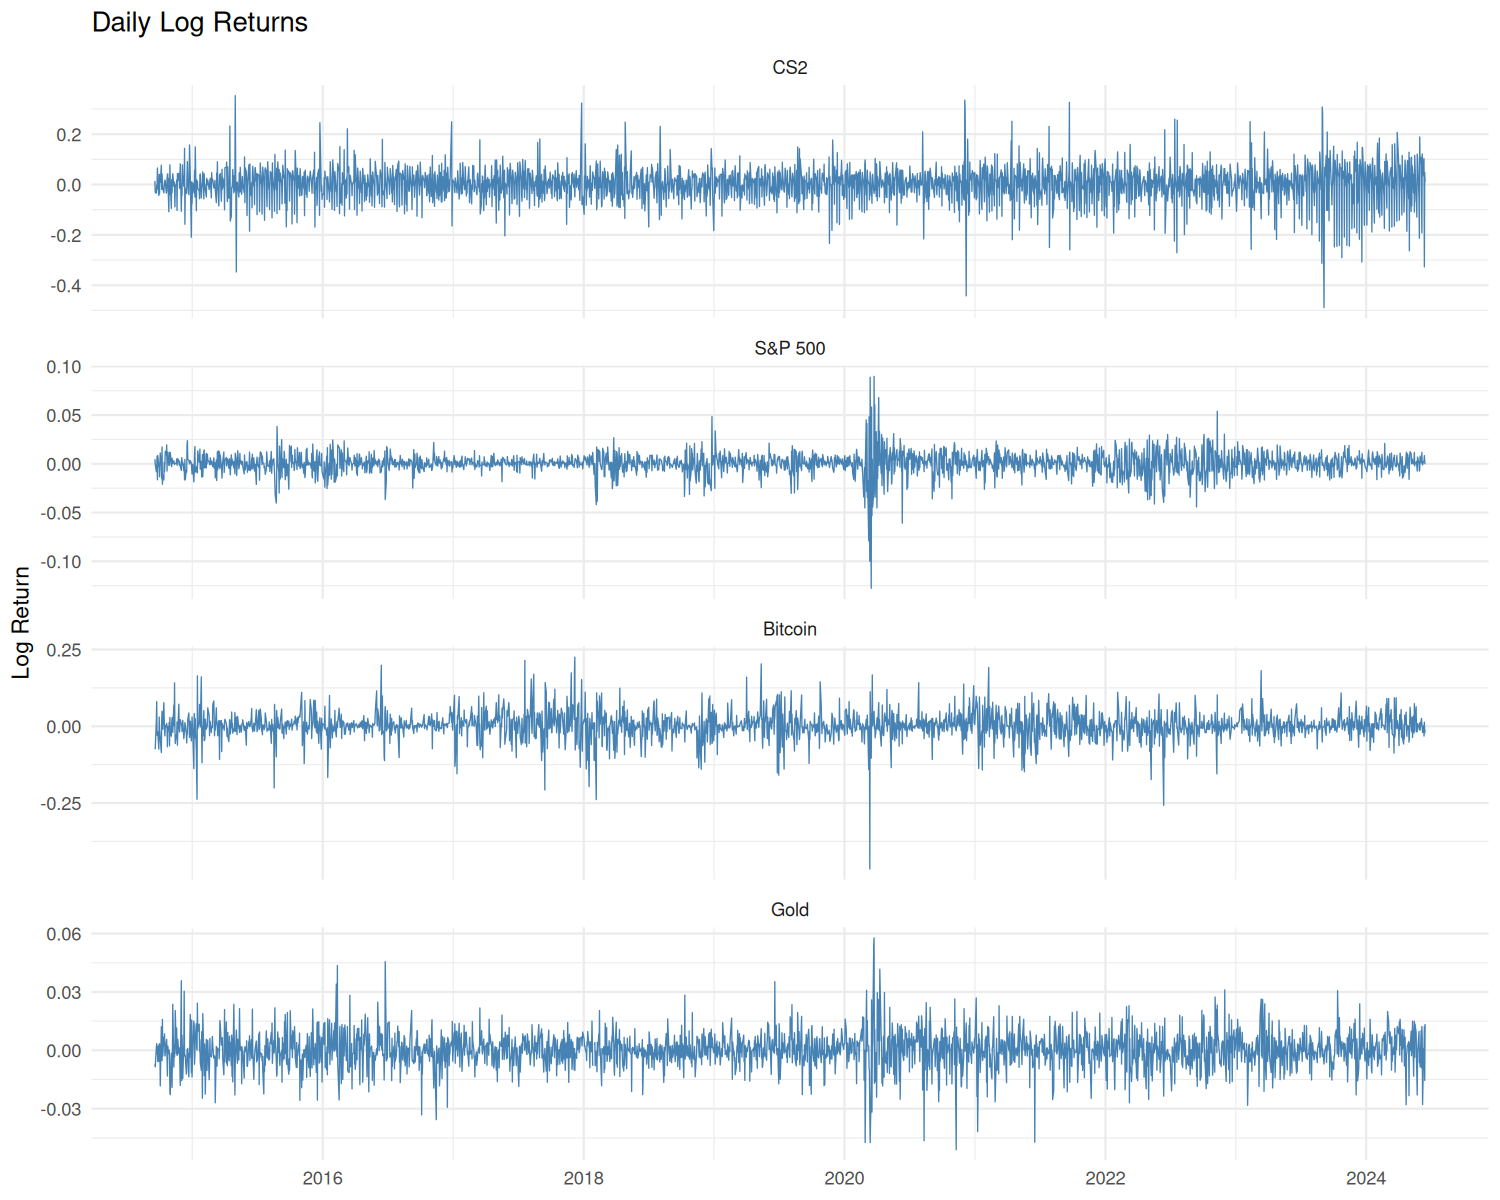
\includegraphics[width=\linewidth]{../images/eda/returns.png}
  \caption{Daily log returns --- CS2 index, S\&P~500, Bitcoin, and Gold
    (2013--2024). CS2 and Bitcoin exhibit substantially wider return swings than
    the S\&P~500 and Gold throughout the sample.}
  \label{fig:returns}
\end{figure}

\subsection{GARCH Volatility Comparison (H3)}
\label{subsec:garch}

Table~\ref{tab:garch} reports estimated GARCH(1,1) parameters. H3 is
\textit{partially supported}. CS2 unconditional volatility (161.88\%) more
than triples the S\&P~500 (49.70\%), confirming the first part. The
unconditional GARCH volatility exceeds the sample standard deviation
(114.56\%) because near-integrated variance ($\hat{\alpha}+\hat{\beta} =
0.9990$) implies a high model-implied long-run variance that the finite sample
mean only partially captures. Turning to volatility dynamics, CS2 and Bitcoin
share identical total persistence ($\hat{\alpha}+\hat{\beta} = 0.9990$),
meaning shocks to both markets decay at the same long-run rate. However, the
decomposition reveals fundamentally different intraday mechanisms: CS2's ARCH
coefficient ($\hat{\alpha} = 0.0151$) is an order of magnitude below Bitcoin's
(0.1265), meaning CS2 volatility barely reacts to individual return shocks but
instead persists in long-duration regimes driven by the GARCH term
($\hat{\beta} = 0.9839$). Bitcoin, by contrast, spikes sharply after each
shock and decays from a higher peak. This distinction --- equal long-run
persistence but qualitatively different shock-response profiles --- is
consistent with the Steam Marketplace's closed trading hours, illiquid order
book, and slow information transmission, which suppress short-term reactivity
while allowing elevated variance states to persist.

\begin{table}[H]
\centering
\caption{GARCH(1,1) Estimates}
\label{tab:garch}
\begin{tabular}{lrrrr}
\hline
Asset    & $\hat{\alpha}$ & $\hat{\beta}$ & $\hat{\alpha}+\hat{\beta}$ & Uncond.\ Vol.\ (\%) \\
\hline
CS2      & 0.0151 & 0.9839 & 0.9990 & 161.88 \\
S\&P 500 & 0.1821 & 0.8158 & 0.9979 &  49.70 \\
Bitcoin  & 0.1265 & 0.8725 & 0.9990 & 337.76 \\
Gold     & 0.0280 & 0.9642 & 0.9923 &  16.61 \\
\hline
\end{tabular}
\end{table}

\subsection{VAR and Granger Causality (H1, H2)}

A VAR(4) model is estimated on the joint system (BIC criterion; AIC suggests
$p = 9$). Table~\ref{tab:granger} reports Granger causality F-tests; each row
tests whether the cause variable Granger-causes the \emph{entire remaining
system jointly}.

\begin{table}[H]
\centering
\caption{Granger Causality Tests --- VAR(4)}
\label{tab:granger}
\begin{tabular}{lrrl}
\hline
Cause variable & F-statistic & $p$-value & Conclusion \\
\hline
Bitcoin  & 1.453 & 0.134 & Not significant \\
S\&P 500 & 1.275 & 0.226 & Not significant \\
Gold     & 1.353 & 0.181 & Not significant \\
CS2      & 1.663 & 0.068 & Not significant (borderline) \\
\hline
\end{tabular}
\end{table}

H1 is \textbf{rejected} on the basis of the correlation matrix (Table~\ref{tab:correlation}):
contemporaneous co-movement with all three benchmarks is indistinguishable from
zero. H2 is \textbf{rejected} by the Granger tests: Bitcoin does not predict
the joint system at any conventional significance level ($p = 0.134$), and the
reverse direction is also non-significant. The borderline CS2 signal ($p =
0.068$) is noteworthy: while below the 5\% threshold, it runs in the opposite
direction to H2, suggesting that if any linear predictive link exists, it flows
\emph{from} CS2 to the broader system rather than towards it. Given that the
test is joint, it is not possible to attribute this signal to any single
benchmark series. Together, the absence of contemporaneous correlation and
dynamic Granger predictability position CS2 as a genuinely segmented market
whose price dynamics are driven by game-specific factors --- patch updates,
tournament cycles, case releases --- rather than by macroeconomic or crypto
forces.

\subsection{Critical Discussion}

The most direct explanation for the low co-movement is informational isolation:
CS2 skin prices respond to game-specific news --- case releases, patch updates,
tournament activity, and developer announcements --- rather than to
macroeconomic or crypto signals. The Steam Marketplace's 15\% transaction fee
reinforces this by making arbitrage between the skin market and other asset
classes prohibitively costly, while the inability to short-sell skins prevents
price-correcting flows from external markets. Ljung-Box tests on VAR(4)
residuals (Table~\ref{tab:ljungbox}) reveal significant residual autocorrelation
in the CS2 and S\&P~500 equations ($Q(10) > 90$, $p < 0.001$), indicating that
VAR(4) does not fully capture CS2's dynamics. However, this misspecification
biases toward conservative inference: residual autocorrelation inflates standard
errors and makes it harder to reject the null of no Granger causality. A
correctly specified, higher-lag model would therefore be even less likely to find
significance. The value-weighted index concentrates on high-volume skins,
suppressing mean returns relative to an equal-weighted benchmark and partly
explaining the low mean return (0.009\%/day) relative to
\citeauthor{dobrynskaya2025videogame}'s 41\% annual figure
\cite{dobrynskaya2025videogame}. The September 2023 CS2 engine update may have
introduced a structural break not captured by the constant-parameter models.
Finally, the joint Granger specification is conservative; a pairwise CS2--Bitcoin
VAR would provide a more focused robustness check for H2.
